%todo: 
%	centrar los inputminted
%	
\documentclass{beamer}
\usepackage[spanish]{babel}
\usepackage[utf8]{inputenc}
\usepackage{minted}
\usepackage{graphicx}
\usepackage{tikz}
\usepackage{smartdiagram}
\usetikzlibrary{trees}

\tikzstyle{every node}=[draw=black,thick,anchor=west]
\tikzstyle{selected}=[draw=red,fill=red!30]
\tikzstyle{optional}=[dashed,fill=gray!50]

\newcommand\TBox[2][]{%
  \tikz\node[draw,ultra thick,align=left,#1] {#2};\hskip2pt}

\makeatletter
\newcommand*{\centerfloat}{%
  \parindent \z@
  \leftskip \z@ \@plus 1fil \@minus \textwidth
  \rightskip\leftskip
  \parfillskip \z@skip}
\makeatother



\mode<presentation> {

% The Beamer class comes with a number of default slide themes
% which change the colors and layouts of slides. Below this is a list
% of all the themes, uncomment each in turn to see what they look like.

\usetheme{default}
%\usetheme{AnnArbor}
%\usetheme{Antibes}
%\usetheme{Bergen}
%\usetheme{Berkeley}
%\usetheme{Berlin}
%\usetheme{Boadilla}
%\usetheme{CambridgeUS}
%\usetheme{Copenhagen}
%\usetheme{Darmstadt}
%\usetheme{Dresden}
%\usetheme{Frankfurt}
%\usetheme{Goettingen}
%\usetheme{Hannover}
%\usetheme{Ilmenau}
%\usetheme{JuanLesPins}
%\usetheme{Luebeck}
%\usetheme{Madrid}
%\usetheme{Malmoe}
%\usetheme{Marburg}
%\usetheme{Montpellier}
%\usetheme{PaloAlto}
%\usetheme{Pittsburgh}
%\usetheme{Rochester}
%\usetheme{Singapore}
%\usetheme{Szeged}
%\usetheme{Warsaw}

% As well as themes, the Beamer class has a number of color themes
% for any slide theme. Uncomment each of these in turn to see how it
% changes the colors of your current slide theme.

%\usecolortheme{albatross}
%\usecolortheme{beaver}
%\usecolortheme{beetle}
%\usecolortheme{crane}
%\usecolortheme{dolphin}
%\usecolortheme{dove}
%\usecolortheme{fly}
%\usecolortheme{lily}
%\usecolortheme{orchid}
%\usecolortheme{rose}
%\usecolortheme{seagull}
%\usecolortheme{seahorse}
%\usecolortheme{whale}
%\usecolortheme{wolverine}

%\setbeamertemplate{footline} % To remove the footer line in all slides uncomment this line
%\setbeamertemplate{footline}[page number] % To replace the footer line in all slides with a simple slide count uncomment this line

%\setbeamertemplate{navigation symbols}{} % To remove the navigation symbols from the bottom of all slides uncomment this line
}

\usepackage{graphicx} % Allows including images
\usepackage{booktabs} % Allows the use of \toprule, \midrule and \bottomrule in tables

%----------------------------------------------------------------------------------------
%	TITLE PAGE
%----------------------------------------------------------------------------------------

\title{Conversión de modelos PowerDEVS al lenguaje Modelica} % The short title appears at the bottom of every slide, the full title is only on the title page

\author{Luciano Andrade} % Your name
\institute[UNR] % Your institution as it will appear on the bottom of every slide, may be shorthand to save space
{
Universidad Nacional de Rosario\\ % Your institution for the title page
\medskip
\textit{andrade.luciano@gmail.com} % Your email address
}
\date{\today} % Date, can be changed to a custom date

\begin{document}


\newcommand{\quotes}[1]{``#1''}

\begin{frame}
\titlepage % Print the title page as the first slide
\end{frame}

\begin{frame}
\frametitle{Overview} % Table of contents slide, comment this block out to remove it
\tableofcontents % Throughout your presentation, if you choose to use \section{} and \subsection{} commands, these will automatically be printed on this slide as an overview of your presentation
\end{frame}

\chapter{Introducción}
\section{Motivación}

\begin{frame}
\begin{itemize}
	\item El sistema físico no se encuentra construido.
	
	\item El experimento puede ser peligroso.

	\item El costo del experimento es demasiado alto.

	\item Los tiempos del sistema no son compatibles con los tiempos del experimentador.
\end{itemize}
\end{frame}

\begin{frame}
\begin{itemize}
	\item Variables de control, de estado y/o del sistema pueden no ser accesibles. 

	\item Eliminación de perturbaciones.

	\item Eliminación de efectos de segundo orden. 
\end{itemize}
\end{frame}

\begin{frame}
\begin{figure}[H]
\centering
 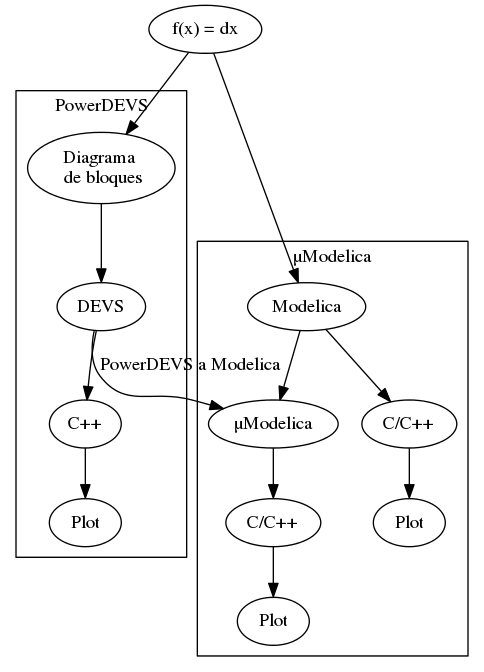
\includegraphics[width=0.50\linewidth]{esquema}
 \caption{Esquema de conversiones}
 \label{fig:esquema}
\end{figure}
\end{frame}

\section{Trabajo relacionado}
\begin{frame}
\begin{itemize}
	\item QSS-Solver
	\item DESlib
	\item M/CD++ 
\end{itemize}
\end{frame}

\chapter{Conceptos Previos}
\section{Modelado y Simulación}
\subsection{Sistemas Continuos y Discretos}
\begin{frame}
	\begin{equation} \label{eq:eq1}
	\dot{x}(t) = f (x(t), u(t))
	\end{equation}

	Con condiciones iniciales :
	\begin{equation} \label{eq:eq2}
	x(t = t_0 ) = x_0
	\end{equation}
\end{frame}

\subsection{Métodos de Integración}
\begin{frame}
	Sea $x_i (t)$ la trayectoria del estado $i$-esimo expresada como función de tiempo simulado. 
	Mientras que la ecuación  \ref{eq:eq1} no contenga discontinuidades $x_i (t)$ será una función continua con derivada continua. 
	Esta puede ser aproximada con la precisión deseada mediante series de Taylor en cualquier punto de su trayectoria.

	\begin{equation} \label{eq3}
		x_i(t^* + h) = x_i(t^*) + \frac{dx_i (t^*)}{dt} \cdot h + \frac{d^{2}x_i (t^*)}{dt^2} \cdot \frac{h^2}{2!} + \cdots
	\end{equation}

	\begin{equation} \label{eq4}
		x_i(t^* + h) = x_i(t^*) + f_i(t^*) \cdot h + \frac{d^{2}x_i (t^*)}{dt^2} \cdot \frac{h^2}{2!} + \cdots
	\end{equation}
\end{frame}

\subsection{Lotka Volterra}
\begin{frame}
	\begin{align*}
		\frac{dx}{dt} &= x(\alpha - \beta y) \\
		\frac{dy}{dt} &= - y(\gamma - \delta  x)
	\end{align*}
	donde:
	\begin{itemize}
		\item $y$ es el número de algún predador (por ejemplo, un lobo)
		\item $x$ es el número de sus presas (por ejemplo, conejos)
		\item $\frac{dy}{dt}$ y $\frac{dx}{dt}$ representa el crecimiento de las dos poblaciones en el tiempo
		\item $t$ representa el tiempo y
		\item $\alpha$, $\beta$, $\gamma$ y $\delta$ son parámetros que representan las interacciones de las dos especies.
	\end{itemize}
\end{frame}

%The prey are assumed to have an unlimited food supply, and to reproduce exponentially unless subject to predation; this exponential growth is represented in the equation above by the term αx. The rate of predation upon the prey is assumed to be proportional to the rate at which the predators and the prey meet; this is represented above by βxy. If either x or y is zero then there can be no predation.

%In this equation,  \displaystyle \delta xy represents the growth of the predator population. (Note the similarity to the predation rate; however, a different constant is used as the rate at which the predator population grows is not necessarily equal to the rate at which it consumes the prey). \displaystyle \gamma y represents the loss rate of the predators due to either natural death or emigration; it leads to an exponential decay in the absence of prey.

\section{Modelica}
\begin{frame}[fragile]
\centering
\begin{listing}[H]    
	\inputminted[linenos]{modelica}{src/LotkaVolterra.mo}
	\caption{LotkaVolterra.mo}\label{lst:LotkaVolterra.mo}
\end{listing}
\end{frame}

\section{Métodos de Integración QSS}
\begin{frame}
	Formalmente, el método de QSS de primer orden (llamado QSS1) aproxima la ecuación por:
	
	\begin{equation}
	\dot{x}(t) = f (q(t), v(t))
	\end{equation}
	
	donde $q$ es el vector de estados cuantificados y sus componentes están relacionadas una a una con las del vector de estados $x$ siguiendo una 
	función de cuantificación con histéresis:
	
	\begin{equation}
	q_j(t) = \left\{ 
	  \begin{array}{l l}
	    x_j(t)  \quad \text{si} \mid x_j (t ) - q_j (t^{-} ) \mid \geq \Delta Q_j \\
	    q_j (t^{-} ) \quad \text{en caso contrario}
	  \end{array} \right.
	\end{equation}
	
	donde $q_j (t^{-})$ es el límite por izquierda de $q_j$ en $t$.
\end{frame}

\begin{frame}
	\begin{figure}[H]
	  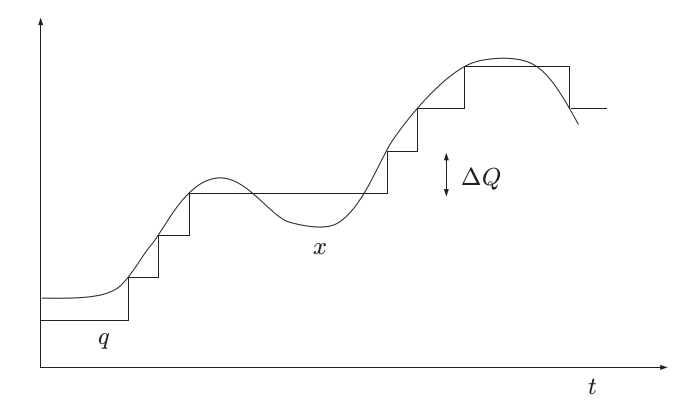
\includegraphics[scale=0.5]{histeresis1}
	  \caption{Variables Relacionadas con una Función de Cuantificación con Histéresis de orden cero.} \label{fig:fig2-2}
	\end{figure}
\end{frame}


\section{$\mu$-Modelica}
\begin{frame}
	\begin{itemize}
	 \item El modelo es plano, es decir no permite clases.
	 \item Todas las variables pertenecen al tipo predefinido Real y solo hay tres categorías de variables: estado continuo, estado discreto y variables 
	algebraicas.
	 \item Los parámetros también son de tipo Real. 
	 \item 
     
    Solo Arreglos unidimensionales están permitidos. Indices en los arreglos dentro de cláusulas \texttt{for} están restringidos a la forma $\alpha \cdot i + \beta$, 
	donde $\alpha$ y $\beta$ son expresiones enteras e \texttt{i} es el índice de la iteración.
	 \item La sección de ecuaciones está compuesta de :
	 \begin{itemize}
		\item Definición de variables de estados : $der(x) =  f (x(t), d, a(t), t);$ ODE en forma explícita
		\item Definición algebraica : $a_2  = g(a_1);$
	 \end{itemize}
	 con la restricción de que cada variable algebraica solo puede depender de variables estado y de variables algebraicas previamente definidas.
	 
	 \item Discontinuidades son expresadas solo con las clausulas $when$ y $elsewhen$ dentro de la sección $algorithm$. Las condiciones dentro de las dos 
	clausulas solo pueden ser relaciones ($<$, $\leqslant$, $>$ $\geqslant$) y, dentro de la clausula, solo asignaciones de variables discretas y $reinit$ 
	de estados continuos son permitidos.
	\end{itemize}
\end{frame}

\section{Stand-Alone QSS-Solver}
\begin{frame}
	\begin{listing}[H]    
		\inputminted[linenos]{modelica}{src/lotka_volterra_qss.mo}
		\caption{LotkaVolterra.mo}\label{lst:LotkaVolterra_qss.mo}
	\end{listing} 
\end{frame}


\section{Formalismo DEVS}
\subsection{Modelos Atómicos}
\begin{frame}
Un modelo atómico representa la unidad \quotes{indivisible} de especificación, en el sentido que es la pieza fundamental y más básica de un modelo DEVS. 
	Formalmente un modelo atómico está conformado por la 7-upla:

	\begin{equation} 
	(X, Y, S, \delta_{int} , \delta_{ext}, \lambda, t_{a}) \mbox{ donde :}
	\end{equation}

	\begin{itemize}
	\item $X$ es el conjunto de valores de entrada que acepta el modelo atómico, es decir un evento de entrada tiene como valor un elemento del conjunto X.
	\item $Y$ es el conjunto de valores de los eventos de salida que puede emitir el modelo atómico.
	\item $S$ es el conjunto de estados internos del modelo, en todo momento el atómico está en un estado dado, que es un elemento del conjunto S.
	\item $ta$ es una función $S \to \mathbb{R}^{+}_{0}$ , que indica cuánto tiempo el modelo atómico permanecerá en un estado dado, si es que no se recibe ningún 
	evento de entrada. Esta función es \emph{Función de Avance de Tiempo}.
	\item $\delta_{int}$ es una función $S \to S$, que indica la dinámica del sistema en el momento que el modelo atómico realiza una transición interna. 
	Sería el análogo a una tabla de transición en otros autómatas, es la \emph{Función de Transición Interna}.
	\item $\delta_{ext}$ es una función $(S \times \mathcal{P}(\mathbb{R}^{+}_{0}) \times X) \to S$, que indica el cambio de estado ante la presencia de un evento 
	externo, esta es la \emph{Función de Transición Externa}.
	\item $\lambda$ es una función $S \to Y$ que indica qué evento se debe emitir al salir de un estado dado, es \emph{Función de Salida}.
	\end{itemize}
\end{frame}

\begin{frame}
	\begin{figure}[H]
	  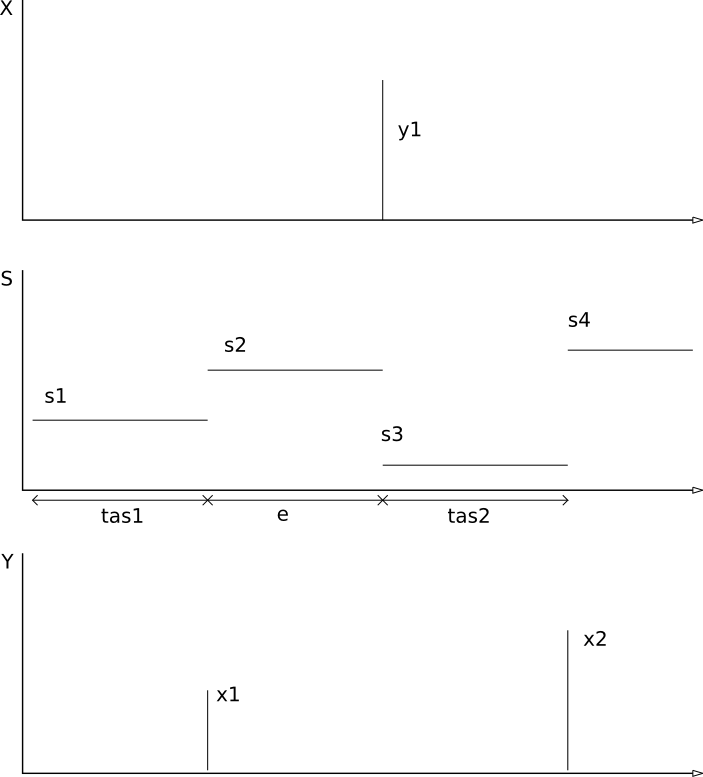
\includegraphics[scale=0.5]{devs-atomic}
	  \caption{Comportamiento de un modelo DEVS atómico}
	   \label{fig:fig2-5}
	\end{figure}
\end{frame}


\subsection{Modelos Acoplados}
\begin{frame}[fragile]
	\begin{figure}[H]
	\begin{minipage}{0.5\textwidth}
	\centering
	\TBox{%
	  \TBox[]{Acoplado2 \\ \TBox{Acoplado1 \\ \TBox[]{Atómico1}\TBox{Atómico2} } \TBox{Atómico3} }}
	\end{minipage}\hfill
	\begin{minipage}{0.5\textwidth}
	\centering

	\begin{tikzpicture}[%
	  grow via three points={one child at (0.5,-0.7) and
	  two children at (0.5,-0.7) and (0.5,-1.4)},
	  edge from parent path={(\tikzparentnode.south) |- (\tikzchildnode.west)}]
	  \node {Root-Coordinator}
	    child { node {Acoplado2}		
	    child { node {Acoplado1}
	      child { node {Atómico1}}
	      child { node {Atómico2}}
	    }
	    child [missing] {}				
	    child [missing] {}				
	    child [missing] {}				
	    child { node {Atómico3}}};
	\end{tikzpicture}
	\end{minipage}

	\caption{Ejemplo de un modelo jerárquico.}\label{jerarquia}

	\end{figure}
\end{frame}

\subsection{Modelos DEVS Parametrizados}
\begin{frame}
	\begin{equation}
	M (p) = \{X, Y, S, \delta_{int}, \delta_{ext} ,\lambda , ta, p\}
	\end{equation}

	donde $p \in P$ es un parámetro que pertenece a un conjunto de parámetros arbitrario tal que $\delta_{int}$ , $\delta_{ext}$ , $\lambda$ y $ta$ 
	dependen también de $p$.
	Notar que dos modelos DEVS $M (p_1 )$, $M (p_2 )$ con $p_1 \neq p_2$ pueden exhibir distintos comportamientos aunque compartan los mismos conjuntos 
	de entrada, salida y de estados ($X$, $Y$ , y $S$, respectivamente).

\end{frame}

\subsection{Modelos Vectoriales}
\begin{frame}
	\begin{equation}
		M (p) = \{X, Y, S, \lambda_{int} , \lambda_{ext} , \lambda, ta, p\}
	\end{equation}

	definimos un modelo Vectorial DEVS\ como la estructura:
	\begin{equation}
		V_D = \{N, X_V, Y_V, P, \{M_i\}\},
	\end{equation}
	donde:
	\begin{itemize}
		\item $N \in \mathbb{N}$ es la dimensión del modelo vectorial.

		\item $X_V = X \times Index \bigcup \{-1\}$ es el conjunto de eventos de entradas vectorial donde $X$ es el conjunto de eventos de entrada del modelo 
		escalar e $Index = {1, \ldots , N }$ es el conjunto de índices que indican cuál de los modelos DEVS atómicos recibirá el evento.

		\item $Y_V = Y \times Index$ es el conjunto de eventos de salida vectorial donde $Y$ es el conjunto de eventos de salida del modelo escalar e 
		$Index = {1, \ldots , N }$ es el conjunto de índices que indica que modelo escalar de los $N$ , emitió el evento. 

		\item $P$ es un conjunto de parámetros arbitrario.

		\item Para cada índice $i \in Index$, $p(i) \in P$ es un parámetro y $M_i = M (p(i))$ es el modelo DEVS Parametrizado escalar.
	\end{itemize}
\end{frame}


\subsubsection{Interfaz entre DEVS Vectorial y DEVS}
\begin{frame}
	\begin{itemize}
		\item Escalar a Vector (Scalar to Vector): Este bloque simplemente agrega al indice $i$ al evento escalar que recibe, transformándolo en un 
			evento vectorial. Este modelo también posee un comportamiento especial para enviar el mismo evento en todas las componentes vectorial 
			al mismo tiempo, cuando $i = -1$, cada evento de entrada es trasmitido para todas las componentes del vector salida.
		\item Vector a escalar (Vector to Scalar): Este bloque tiene un parámetro $i$ que contiene el índice del vector de eventos a retransmitir, 
			cuando recibe un evento con indice $j=i$, remueve el indice y retransmite el evento escalar.
		\item Index Shift: El modelo más simple es el Index Shift. Cuando se recibe un evento con el valor $(x,i)$, emite un evento de salida $(x, i+sh)$, 
			donde $sh$ es un parámetro entero.
	\end{itemize}
\end{frame}

\section{PowerDEVS}
\begin{frame}
	\begin{figure}[H]
	  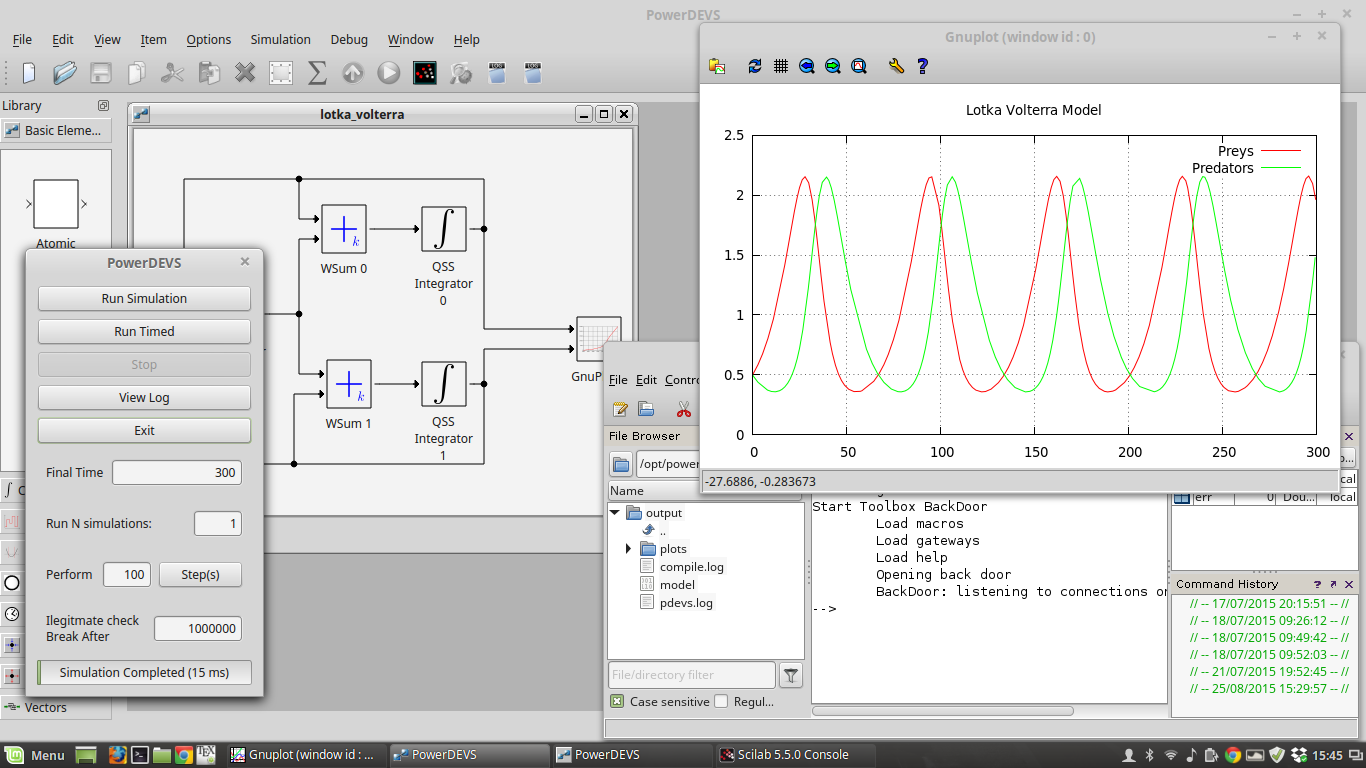
\includegraphics[width=\textwidth]{powerdevs}
	  \caption{Interfaz gráfica de PowerDEVS}
	   \label{fig:powerdevsgui}
	\end{figure}
\end{frame}

\chapter{Conversión de modelos DEVS}
\begin{frame}
\begin{listing}[H]
        \inputminted[linenos,breaklines=true,lastline=32]{modelica}{src/lotka_volterra.pds}
\caption{Estructura del archivo lotka\_volterra.pds, modelos atómicos (continua).}\label{lst:pdsstruc}
\end{listing}
\end{frame}

\begin{frame}
\begin{listing}[H]
        \inputminted[firstline=33,linenos,breaklines=true]{modelica}{src/lotka_volterra.pds}
\caption{(continuación) conexiones del archivo lotka\_volterra.pds.}\label{lst:pdsstruc-cont}
\end{listing}
\end{frame}

\section{Modelos DEVS}
\subsection{Archivos PDS}
\begin{frame}
\begin{listing}[H]
        \inputminted[linenos,breaklines=true,lastline=32]{modelica}{src/lotka_volterra.pds}
\caption{Estructura del archivo lotka\_volterra.pds, modelos atómicos (continua).}\label{lst:pdsstruc}
\end{listing}
\end{frame}

\begin{frame}
\begin{listing}[H]
        \inputminted[firstline=33,linenos,breaklines=true]{modelica}{src/lotka_volterra.pds}
\caption{(continuación) conexiones del archivo lotka\_volterra.pds.}\label{lst:pdsstruc-cont}
\end{listing}
\end{frame}

\section{Modelos Atómicos}
\subsection{Modelos Continuos}
\begin{frame}
\begin{listing}[H]
        \inputminted[]{modelica}{../../data/qss/qss_wsum.mo}
        \caption{Modelo atómico sumador}\label{lst:qss_wsum.mo}
\end{listing}
\end{frame}

\subsection{Modelos Discontinuos}
\begin{frame}[fragile]
\begin{listing}[H]
        \inputminted[]{modelica}{../../data/qss/qss_switch.mo}
        \caption{Modelo atómico Switch}\label{lst:qss_switch.mo}
\end{listing}
\end{frame}

\subsection{Protocolo}
\begin{frame}[fragile]
\begin{itemize}
        \item El código debe ser Modelica ($\mu$-modelica) válido y estar ubicado en el mismo directorio (y nombre del archivo) del código C que el modelo atómico 
        PowerDEVS, con el mismo nombre que el archivo .h, pero con extensión .mo, es decir un modelo con \texttt{vector\textbackslash qss\_sum\_vec.h} 
	utilizará un modelo \texttt{vector/qss\_sum\_vec.h} \footnote{El nombre de los archivos se remplaza \quotes{\textbackslash} por \quotes{/} para permitir 
	algunos modelos cuyos \texttt{Path} contiene ese separadores de directorios}
        \item Los parámetros del modelo DEVS deben ser pasado en el parámetro $p$, el cual es un arreglo de reales. 
        \item Los valores de entrada del modelo son asociados a la variable $u$
        \item Los valores de salida del modelos son asociados a la variable $y$
\end{itemize}
\end{frame}

\begin{frame}[fragile]
\begin{minted}{modelica}
class QSSIntegrator
  parameter Real p[4]={0,0,0,0,0,0,0,0};
  parameter Real x0 = p[4];
  Real u[1];
  Real y[1](start = {x0});
equation
  der(y[1]) = u[1];
end QSSIntegrator;
\end{minted}
\end{frame}

\begin{frame}[fragile]
\begin{listing}[H]
\begin{minted}{text}
  ...
  Simulator
   {
    Path = qss/qss_integrator.h
    Parameters = "QSS3","1e-6","1e-3","0.5"
   }
   ...
\end{minted}
\caption{Extracto del modelo Lotka Volterra, modelo atómico de un integrator.}\label{lst:qssint.pds}
\end{listing}
\end{frame}

\begin{frame}[fragile]
\begin{listing}[H]
\begin{minted}{modelica}
class QSSIntegrator
  parameter Real QSSIntegrator_1_p[4]={0,1e-6, 1e-3, 0.5};
  parameter Real QSSIntegrator_1_x0 = p[4];
  Real QSSIntegrator_1_u[1];
  Real QSSIntegrator_1_y[1](start = {QSSIntegrator_1_x0});
equation
  der(QSSIntegrator_1_y[1]) = QSSIntegrator_1_u[1];
end QSSIntegrator;
\end{minted}
\caption{Transformación parcial de un modelo atómico de un integrator en el modelo de ejemplo Lotka Volterra.}\label{lst:integradorparametros}
\end{listing}
\end{frame}

\section{Modelos Acoplados Planos}
\begin{frame}[fragile]
\begin{listing}[H]
        \inputminted[linenos]{modelica}{src/lotka_volterra-orig.mo}
        \caption{Modelo Lotka Volterra convertido de PowerDEVS a $\mu$-Modelica}
        \label{lst:lotka_volterra-orig.mo}
\end{listing}
\end{frame}

\section{Modelos Acoplados Jerárquico}
\begin{frame}
        \begin{itemize}
                \item por cada modelo acoplado si solo tiene modelos atómicos, es remplazado por los modelos atómicos internos, los cuales se encuentran conectados 
                        sin modificaciones excepto por las conexiones externas, las cuales son reasignadas de forma de mantener las conexiones.
                \item si el modelo acoplado contiene otros modelos acoplados entonces aplanamos ese modelo recursivamente.
        \end{itemize} 
\end{frame}

\begin{frame}[fragile]
\begin{figure}[H]
        \begin{minipage}{0.5\textwidth}
        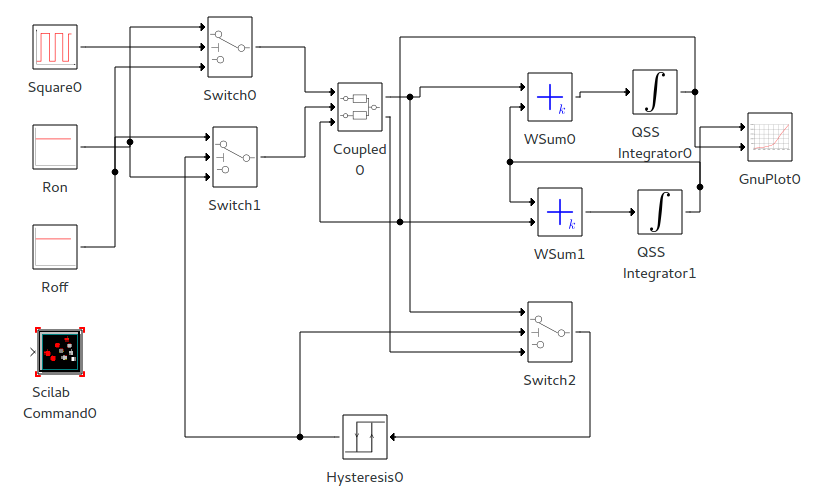
\includegraphics[width=\linewidth]{buck_disk}
        \end{minipage}
        \begin{minipage}{0.5\textwidth}
        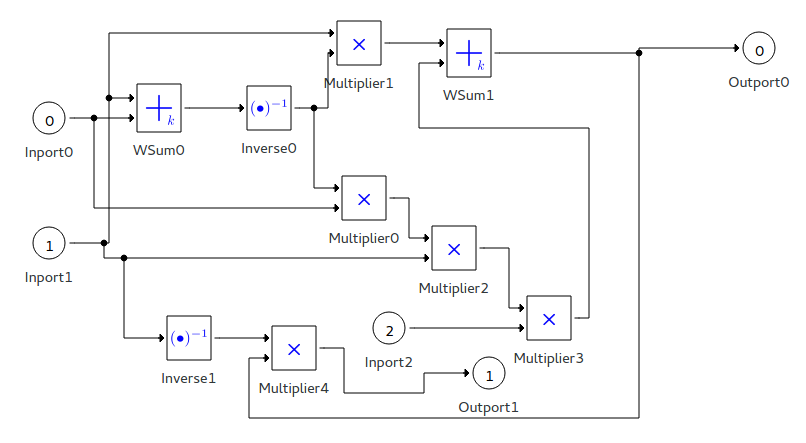
\includegraphics[width=\linewidth]{buck_disk_coupled0}
        \end{minipage}
 \caption{Ejemplo de modelo acoplado(derecha), junto a una detalle del modelo \texttt{Coupled0}}\label{fig:coupledsample}
\end{figure}
\end{frame}

\begin{frame}[fragile]
\begin{figure}[H]
  %\setcapwidth{0.6\textwidth}
  \makebox[\textwidth][c]{%
        \begin{minipage}[t][][b]{.59\textwidth}
        \begin{tikzpicture}[%
          grow via three points={one child at (0.5,-0.7) and
          two children at (0.5,-0.7) and (0.5,-1.4)},
          edge from parent path={(\tikzparentnode.south) |- (\tikzchildnode.west)}]
          \node {Root-Coordinator}
            child { node {Scilab Command0 (0)}}             
            child { node {QSS Integartor0 (1)}}
            child { node {QSS Integartor1 (2)}}             
            child { node {Coupled0        (3)}
              child { node {WSum0       (0)}}
              child { node {Inseverse0  (1)}}
              child { node {Multiplier0 (2)}}
              child { node {Multiplier1 (3)}}
              child { node {Multiplier2 (4)}}
              child { node {Inseverse1  (5)}}
              child { node {Multiplier3 (6)}}
              child { node {Multiplier4 (7)}}
              child { node {WSum1       (8)}}
            }
            child [missing] {}                          
            child [missing] {}                          
            child [missing] {}                          
            child [missing] {}                          
            child [missing] {}                          
            child [missing] {}                          
            child [missing] {}                          
            child [missing] {}                          
            child [missing] {}                          
            child { node {Switch0    (4)}}
            child { node {Ron        (5)}}
            child { node {Roff       (6)}}
            child { node {Square0    (7)}}
            child { node {GNUPlot0   (8)}}
            child { node {Hysteresis0(9)}}
            child { node {Switch1    (10)}}
            child { node {WSum0      (11)}}
            child { node {WSum1      (12)}};
        \end{tikzpicture}
        \end{minipage} %
        \hfill
        \begin{minipage}[t][][b]{.59\textwidth}
        \begin{tikzpicture}[%
          grow via three points={one child at (0.5,-0.7) and
          two children at (0.5,-0.7) and (0.5,-1.4)},
          edge from parent path={(\tikzparentnode.south) |- (\tikzchildnode.west)}]
          \node {Root-Coordinator}
            child { node {Scilab Command0	(0)}}
            child { node {QSS Integartor0	(1)}}
            child { node {QSS Integartor1	(2)}}             
            child { node {WSum0			(3)}}
            child { node {Inseverse0		(4)}}
            child { node {Multiplier0		(5)}}
            child { node {Multiplier1		(6)}}
            child { node {Multiplier2		(7)}}
            child { node {Inseverse1		(8)}}
            child { node {Multiplier3		(9)}}
            child { node {Multiplier4		(10)}}
            child { node {WSum1			(11)}}
            child { node {Switch0		(12)}}
            child { node {Ron			(13)}}
            child { node {Roff			(14)}}
            child { node {Square0		(15)}}
            child { node {GNUPlot0		(16)}}
            child { node {Hysteresis0		(17)}}
            child { node {Switch1		(18)}}
            child { node {WSum0			(19)}}
            child { node {WSum1			(20)}};
        \end{tikzpicture}
        \end{minipage}%
}
        \caption{Modelo convertidor de potencia, jerarquía original (izquierda) y aplanada (derecha), junto al nombre, esta la posición que ocupan dentro del modelo acoplado que los contiene.}
        \label{fig:coupled-tree}
\end{figure}
\end{frame}

\begin{frame}[fragile]
\begin{minipage}[t]{0.5\linewidth}
\centering
\begin{minted}[linenos]{text}
 IC
   {
   (13,0);(1,0)
    (12,0);(2,0)
    (8,0);(4,1)
    (4,0);(3,0)
    (5,0);(3,1)
    (3,1);(11,2)
    (11,0);(10,0)
    (2,0);(9,0)
    (2,0);(12,0)
    (2,0);(13,1)
    (3,0);(11,0)
    (3,0);(13,0)
    (10,0);(11,1)
    (10,0);(5,1)
    (1,0);(3,2)
    (1,0);(12,1)
    (1,0);(9,1)
    (6,0);(5,2)
    (6,0);(4,0)
    (7,0);(5,0)
    (7,0);(4,2)
}
\end{minted}
\end{minipage}
\begin{minipage}[t]{0.5\linewidth}
\begin{minted}[linenos]{text}
     EIC
       {
        (0,2);(4,1)
        (0,0);(2,1)
        (0,0);(0,1)
        (0,1);(3,1)
        (0,1);(5,0)
        (0,1);(7,0)
        (0,1);(0,0)
       }
      EOC
       {
        (6,0);(0,1)
        (8,0);(0,0)
       }
      IC
       {
        (0,0);(1,0)
        (7,0);(8,0)
        (2,0);(3,0)
        (3,0);(4,0)
        (5,0);(6,0)
        (4,0);(8,1)
        (1,0);(2,0)
        (1,0);(7,1)
        (8,0);(6,1)
       }
\end{minted}
\end{minipage}
\end{frame}

\begin{frame}
\begin{itemize}
        \item Conexiones que involucran modelos atómicos ubicados después del modelo acoplado y no están relacionadas con el modelo acoplado, 
        estas conexiones deben ser modificadas dado que insertaremos los modelos atómicos del modelo acoplado que estamos aplanando, y los modelos 
        ubicados después del modelo acoplado serán desplazados.
\end{itemize}
\end{frame}

\begin{frame}[fragile]
\begin{columns}[T] % align columns
\begin{column}{.48\textwidth}
\begin{minted}[linenos]{text}
      IC
        {
         (13,0);(1,0)
         (12,0);(2,0)
         (8,0);(4,1)
         (11,0);(10,0)
         (2,0);(9,0)
         (2,0);(12,0)
         (2,0);(13,1)
         (10,0);(11,1)
         (10,0);(5,1)
         (1,0);(12,1)
         (1,0);(9,1)
         (6,0);(5,2)
         (6,0);(4,0)
         (7,0);(5,0)
         (7,0);(4,2)
       }
\end{minted}
\end{column}%
\hfill%
\begin{column}{.48\textwidth}
\begin{minted}[linenos]{text}
      IC
        {
         (21,0);(1,0)
         (20,0);(2,0)
         (16,0);(12,1)
         (19,0);(18,0)
         (2,0);(17,0)
         (2,0);(20,0)
         (2,0);(21,1)
         (18,0);(19,1)
         (18,0);(13,1)
         (1,0);(20,1)
         (1,0);(17,1)
         (14,0);(13,2)
         (14,0);(12,0)
         (15,0);(13,0)
         (15,0);(12,2)
       }
\end{minted}
\end{column}%
\end{columns}
\end{frame}

\begin{frame}[fragile]
\begin{itemize}
        \item Agregamos las conexiones internas del modelo acoplado que eliminaremos al modelo acoplado \texttt{Root-Coordinator}, estas conexiones deben ser 
        modificadas ya que los modelos atómicos insertados son insertados en la posición del modelo acoplado eliminado.
\end{itemize}
\end{frame}

\begin{frame}[fragile]
\begin{columns}[T] % align columns
\begin{column}{.48\textwidth}
\begin{minted}{text}
      IC
       {
        (0,0);(1,0)
        (7,0);(8,0)
        (2,0);(3,0)
        (3,0);(4,0)
        (5,0);(6,0)
        (4,0);(8,1)
        (1,0);(2,0)
        (1,0);(7,1)
        (8,0);(6,1)
       }
\end{minted}
\end{column}%
\hfill%
\begin{column}{.48\textwidth}
\begin{minted}{text}
      IC
       {
        (3,0);(4,0)
        (10,0);(11,0)
        (5,0);(6,0)
        (6,0);(7,0)
        (8,0);(9,0)
        (7,0);(11,1)
        (4,0);(5,0)
        (4,0);(10,1)
        (11,0);(9,1)
       }
\end{minted}
\end{column}%
\end{columns}
\end{frame}

\begin{frame}
\begin{figure}[H]
\centering
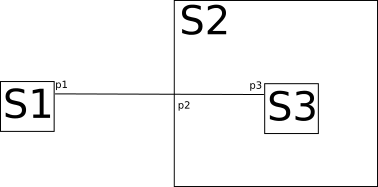
\includegraphics[width=.75\textwidth]{text3418}
\caption{Esquema de conexiones, el modelo \texttt{S1} y \texttt{S3} son modelo atómico, \texttt{S2} es el modelo acoplado que estamos aplanando.\
	\texttt{S1} y \texttt{S2} están conectados a través de los puertos \texttt{p1} y \texttt{p2} respectivamente. Luego, el modelo \texttt{S3} conecta con
	el exterior a través del modelo acoplado que lo contiene por el puerto \texttt{p2} y el puerto  \texttt{p3}.
	} \label{fig:aplanado-ports}
\end{figure}
\end{frame}

\begin{frame}
	\begin{itemize}
	\item IC : \texttt{(S1,p1);(S2,p2)}
	\item EIC : \texttt{(0,p2);(S3,p3)}
	\end{itemize}

	entonces la conexiones en el modelo aplanado es \texttt{($S1$,$p1$);($S3$,$p3$)} y $S1$ debe ser desplazado según la cantidad de modelos que contiene $S2$ y 
	$S3$ deberá ser desplazado según la posición de $S2$.

	Si consideramos que $p2$ es un puerto de salida las conexiones serán:

	\begin{itemize}
	\item IC : \texttt{(S2,p2);(S1,p1)}
	\item EOC : \texttt{(S3,p3);(0,p2)}
	\end{itemize}

	entonces la conexiones en el modelo aplanado es \texttt{($S3$,$p3$);($S1$,$p1$)} e igual que en el caso anterior, $S1$ debe ser desplazado según la 
	cantidad de modelos que contiene $S2$ y $S3$ deberá ser desplazado según la posición de $S2$.
\end{frame}

\begin{frame}[fragile]
\begin{minipage}[t]{0.3\linewidth}
\begin{minted}{text}
      IC
       {
        (3,1);(11,2)
        (3,0);(11,0)
        (3,0);(13,0)
       }
\end{minted}
\end{minipage}
\begin{minipage}[t]{0.3\linewidth}
\begin{minted}{text}
      EOC
       {
        (6,0);(0,1)
        (8,0);(0,0)
       }
\end{minted}
\end{minipage}
\begin{minipage}[t]{0.3\linewidth}
\begin{minted}{text}
      IC
       {
        (9,0);(19,2)
        (11,0);(19,0)
        (11,0);(21,0)
       }
\end{minted}
\end{minipage}
%\caption{Conexiones internas desde el modelo acoplado hacia otro modelo (izquierda), conexiones externas de salida (centro), conexiones internas a agregar al modelo aplanando(derecha).}\label{lst:conecOut}
\end{frame}

\begin{frame}[fragile]
\begin{minipage}[t]{0.3\linewidth}
\begin{minted}{text}
      IC
       {
        (4,0);(3,0)
        (5,0);(3,1)
        (1,0);(3,2)
       }
\end{minted}
\end{minipage}
\begin{minipage}[t]{0.3\linewidth}
\begin{minted}{text}
      EIC
       {
        (0,2);(4,1)
        (0,0);(2,1)
        (0,0);(0,1)
        (0,1);(3,1)
        (0,1);(5,0)
        (0,1);(7,0)
        (0,1);(0,0)
       }
\end{minted}
\end{minipage}
\begin{minipage}[t]{0.3\linewidth}
\begin{minted}{text}
      IC
       {
        (12,0);(5,1)
        (12,0);(3,1)
        (13,0);(6,1)
        (13,0);(8,0)
        (13,0);(10,0)
        (13,0);(3,0)
        (1,0);(7,1)
       }
\end{minted}
\end{minipage}
%\caption{Conexiones internas hacia el modelo acoplado (izquierda), conexiones externas de entrada(centro), conexiones internas a agregar al modelo aplanando(derecha).}
%\label{lst:conecIn}
%\end{listing}
\end{frame}


\section{Modelos Vectoriales}
\begin{frame}
\begin{itemize}
	\item \texttt{annotation(PD2MO = \{Scalar, Scalar\});} entrada y salida son escalares, este es el caso por omisión y no es necesario declararlo.
	\item \texttt{annotation(PD2MO = \{Scalar, Vector\});} entrada escalar y salida vectorial
	\item \texttt{annotation(PD2MO = \{Vector, Scalar\});} entrada escalar y salida vectorial
	\item \texttt{annotation(PD2MO = \{Vector, Vector\});} entrada y salida vectoriales.
\end{itemize}
\end{frame}

	\begin{itemize}
	\item Causalización de variables, este es un programa descripto en \cite{Mod15}
	\item Transformaciones de Modelica a $\mu$-Modelica, si bien existe un programa con esta finalidad, éste no implementa (al momento de escribir este texto)
	las transformaciones que necesitamos por lo que son descriptas en la sección \ref{sec:transform} e involucra las construcciones de Modelica 
		\texttt{if...then...else}, producto interno de dos vectores y arreglos bidimensionales.
	\end{itemize}


\section{Transformaciones Extra}
\begin{frame}
	\begin{itemize}
	\item Causalización de variables, este es un programa descripto en \cite{Mod15}
	\item Transformaciones de Modelica a $\mu$-Modelica, si bien existe un programa con esta finalidad, éste no implementa (al momento de escribir este texto)
	las transformaciones que necesitamos por lo que son descriptas en la sección \ref{sec:transform} e involucra las construcciones de Modelica 
		\texttt{if...then...else}, producto interno de dos vectores y arreglos bidimensionales.
	\end{itemize}
\end{frame}

\section{Preservación de la Semántica}
\begin{frame}
	En caso de las transformaciones extra, no solo se encuentran dentro del mismo lenguaje, sino que las construcciones, \texttt{if...then...else}, 
		producto interno de dos vectores y arreglos bidimensionales, son expandidas según su definición, por lo que conservan la misma semántica.

	Con respecto a la estructura del Modelo PowerDEVS, las conexiones entre los modelos atómicos convierten una o $N$ conexiones en PowerDEVS, en una o $N$
	 igualdades en Modelica, dependiendo si el modelo es escalares o vectoriales. La transformación de conexión a igualdad, es la transformación que más 
	nos sirve, pues por un lado, estamos tratando de eliminar el pasaje de eventos entre puertos para liberar recursos computacionales y
	es una estrategia utilizada en el modelado de sistemas en PowerDEVS.

	El procedimiento de aplanado, es por construcción el procedimiento que sigue el evento según esta conectado, es decir si un modelo $a$, esta conectado
	a un modelo $b$ a través de a un puerto (de entrada o salida), la conexión del modelo aplanado es la conexión entra $a$ y $b$. 

	Por último la traducción entre modelos atómicos como es realizada a mano, y con anticipación a la conversión automática, depende la capacidad de 
	quien realiza esta traducción.
\end{frame}

%	
%	%----------------------------------------------------------------------------------------
%	%	PRESENTATION SLIDES
%	%----------------------------------------------------------------------------------------
%	
%	%------------------------------------------------
%	\section{First Section} % Sections can be created in order to organize your presentation into discrete blocks, all sections and subsections are automatically printed in the table of contents as an overview of the talk
%	%------------------------------------------------
%	
%	\subsection{Subsection Example} % A subsection can be created just before a set of slides with a common theme to further break down your presentation into chunks
%	
%	\begin{frame}
%	\frametitle{Paragraphs of Text}
%	Sed iaculis dapibus gravida. Morbi sed tortor erat, nec interdum arcu. Sed id lorem lectus. Quisque viverra augue id sem ornare non aliquam nibh tristique. Aenean in ligula nisl. Nulla sed tellus ipsum. Donec vestibulum ligula non lorem vulputate fermentum accumsan neque mollis.\\~\\
%	
%	Sed diam enim, sagittis nec condimentum sit amet, ullamcorper sit amet libero. Aliquam vel dui orci, a porta odio. Nullam id suscipit ipsum. Aenean lobortis commodo sem, ut commodo leo gravida vitae. Pellentesque vehicula ante iaculis arcu pretium rutrum eget sit amet purus. Integer ornare nulla quis neque ultrices lobortis. Vestibulum ultrices tincidunt libero, quis commodo erat ullamcorper id.
%	\end{frame}
%	
%	%------------------------------------------------
%	
%	\begin{frame}
%	\frametitle{Bullet Points}
%	\begin{itemize}
%	\item Lorem ipsum dolor sit amet, consectetur adipiscing elit
%	\item Aliquam blandit faucibus nisi, sit amet dapibus enim tempus eu
%	\item Nulla commodo, erat quis gravida posuere, elit lacus lobortis est, quis porttitor odio mauris at libero
%	\item Nam cursus est eget velit posuere pellentesque
%	\item Vestibulum faucibus velit a augue condimentum quis convallis nulla gravida
%	\end{itemize}
%	\end{frame}
%	
%	%------------------------------------------------
%	
%	\begin{frame}
%	\frametitle{Blocks of Highlighted Text}
%	\begin{block}{Block 1}
%	Lorem ipsum dolor sit amet, consectetur adipiscing elit. Integer lectus nisl, ultricies in feugiat rutrum, porttitor sit amet augue. Aliquam ut tortor mauris. Sed volutpat ante purus, quis accumsan dolor.
%	\end{block}
%	
%	\begin{block}{Block 2}
%	Pellentesque sed tellus purus. Class aptent taciti sociosqu ad litora torquent per conubia nostra, per inceptos himenaeos. Vestibulum quis magna at risus dictum tempor eu vitae velit.
%	\end{block}
%	
%	\begin{block}{Block 3}
%	Suspendisse tincidunt sagittis gravida. Curabitur condimentum, enim sed venenatis rutrum, ipsum neque consectetur orci, sed blandit justo nisi ac lacus.
%	\end{block}
%	\end{frame}
%	
%	%------------------------------------------------
%	
%	\begin{frame}
%	\frametitle{Multiple Columns}
%	\begin{columns}[c] % The "c" option specifies centered vertical alignment while the "t" option is used for top vertical alignment
%	
%	\column{.45\textwidth} % Left column and width
%	\textbf{Heading}
%	\begin{enumerate}
%	\item Statement
%	\item Explanation
%	\item Example
%	\end{enumerate}
%	
%	\column{.5\textwidth} % Right column and width
%	Lorem ipsum dolor sit amet, consectetur adipiscing elit. Integer lectus nisl, ultricies in feugiat rutrum, porttitor sit amet augue. Aliquam ut tortor mauris. Sed volutpat ante purus, quis accumsan dolor.
%	
%	\end{columns}
%	\end{frame}
%	
%	%------------------------------------------------
%	\section{Second Section}
%	%------------------------------------------------
%	
%	\begin{frame}
%	\frametitle{Table}
%	\begin{table}
%	\begin{tabular}{l l l}
%	\toprule
%	\textbf{Treatments} & \textbf{Response 1} & \textbf{Response 2}\\
%	\midrule
%	Treatment 1 & 0.0003262 & 0.562 \\
%	Treatment 2 & 0.0015681 & 0.910 \\
%	Treatment 3 & 0.0009271 & 0.296 \\
%	\bottomrule
%	\end{tabular}
%	\caption{Table caption}
%	\end{table}
%	\end{frame}
%	
%	%------------------------------------------------
%	
%	\begin{frame}
%	\frametitle{Theorem}
%	\begin{theorem}[Mass--energy equivalence]
%	$E = mc^2$
%	\end{theorem}
%	\end{frame}
%	
%	%------------------------------------------------
%	
%	\begin{frame}[fragile] % Need to use the fragile option when verbatim is used in the slide
%	\frametitle{Verbatim}
%	\begin{example}[Theorem Slide Code]
%	\begin{verbatim}
%	\begin{frame}
%	\frametitle{Theorem}
%	\begin{theorem}[Mass--energy equivalence]
%	$E = mc^2$
%	\end{theorem}
%	\end{frame}\end{verbatim}
%	\end{example}
%	\end{frame}
%	
%	%------------------------------------------------
%	
%	\begin{frame}
%	\frametitle{Figure}
%	Uncomment the code on this slide to include your own image from the same directory as the template .TeX file.
%	%\begin{figure}
%	%\includegraphics[width=0.8\linewidth]{test}
%	%\end{figure}
%	\end{frame}
%	
%	%------------------------------------------------
%	
%	\begin{frame}[fragile] % Need to use the fragile option when verbatim is used in the slide
%	\frametitle{Citation}
%	An example of the \verb|\cite| command to cite within the presentation:\\~
%	
%	This statement requires citation \cite{p1}.
%	\end{frame}
%	
%	%------------------------------------------------
%	
%	\begin{frame}
%	\frametitle{References}
%	\footnotesize{
%	\begin{thebibliography}{99} % Beamer does not support BibTeX so references must be inserted manually as below
%	\bibitem[Smith, 2012]{p1} John Smith (2012)
%	\newblock Title of the publication
%	\newblock \emph{Journal Name} 12(3), 45 -- 678.
%	\end{thebibliography}
%	}
%	\end{frame}
%	
%	%------------------------------------------------
%	
%	\begin{frame}
%	\Huge{\centerline{The End}}
%	\end{frame}
%	
%----------------------------------------------------------------------------------------

\end{document}
